\documentclass[a4paper,10pt
,draft
%, final
]{article}%





% ---- Commands on draft --------

\usepackage[dvipsnames]{xcolor}% adds colors
\usepackage{ifdraft}[pos=0.8]
\ifdraft{
  \color[RGB]{63,63,63}
  \pagecolor[RGB]{220,220,204}
  \usepackage[notref]{showkeys}
  \usepackage{todonotes}
}
{
  \usepackage[disable]{todonotes}
}

\pdfcompresslevel=0
\pdfobjcompresslevel=0


\usepackage{xr-hyper} % for \externaldocument
\externaldocument[OC-]{OneColor} % cite using names from other half
\externaldocument[AC-]{AllColors} % cite using names from other half
\externaldocument[TAS-]{TameAndSquare} % cite using names from other half


\usepackage[pagebackref, colorlinks, citecolor=PineGreen, linkcolor=PineGreen]{hyperref}
\hypersetup{
  final,
  pdftitle={Left adjoint to the operadic homotopy coherent nerve},
  pdfauthor={Bonventre, P. and Pereira, L. A.},
  linktoc=page,
  pdfpagemode=UseNone,
  pdfpagelayout=SinglePage,
}






\usepackage{amsmath, amsthm}% {amsfonts, amssymb}

% ------ New Characters --------------------------------------

\let\llhook\lhook
\usepackage[latin1]{inputenc}%
%\usepackage[T1]{fontenc}
\usepackage{MnSymbol}
\usepackage[
cal = cm,
bb = ams,
frak = euler,
scr = rsfs
]{mathalpha}

% \DeclareMathAlphabet\mathbb{U}{msb}{m}{n}
% %\usepackage{stmaryrd}
% %\usepackage{upgreek}
% \usepackage{mathrsfs}
% % \usepackage[english]{babel}
% % \usepackage{fouriernc}
% % \DeclareMathAlphabet{\mathscr}{U}{mathrsfs}{m}{n}`
% %\usepackage{pifont}
% %\newcommand{\cmark}{\text{\ding{51}}}
% %\newcommand{\xmark}{\text{\ding{55}}}

\usepackage[normalem]{ulem} % underlining
% \usepackage{dsfont} % double strike-through
% \usepackage{bbm} % more blackboard bold



%----- Enumerate ---------------------------------------------
% \usepackage{paralist} % for inparaenum
% \usepackage{enumerate}%
\usepackage[inline,shortlabels]{enumitem}%
\setenumerate{label=(\roman*)}

% ---------- Page Typesetting ----------
\usepackage[final]{microtype}
\usepackage{relsize}
\usepackage{geometry}

%-------- Tikz ---------------------------

\usepackage{tikz}%
\usetikzlibrary{matrix,arrows,decorations.pathmorphing,
cd,patterns,calc}
\tikzset{%
  % treenode/.style = {shape=rectangle, rounded corners, draw, align=center, font=\footnotesize,
  %                    top color=white, bottom color=blue!20},%
  % root/.style     = {treenode, font=\Large, bottom color=red!30},%
  % env/.style      = {treenode, font=\ttfamily\normalsize},%
  dummy/.style    = {circle,draw,inner sep=0pt,minimum size=2mm}%
}%

\usetikzlibrary[decorations.pathreplacing]




% ----- Labels Changed? --------

\makeatletter

\def\@testdef #1#2#3{%
  \def\reserved@a{#3}\expandafter \ifx \csname #1@#2\endcsname
  \reserved@a  \else
  \typeout{^^Jlabel #2 changed:^^J%
    \meaning\reserved@a^^J%
    \expandafter\meaning\csname #1@#2\endcsname^^J}%
  \@tempswatrue \fi}

\makeatother

%%%%%%%%%%%%%%%%%%%%%%%%% INTERNAL REFERENCES %%%%%%%%%%%%%%%%%%%%%%%%%%%%%%%%%%%

\numberwithin{equation}{section} 
\numberwithin{figure}{section}

\usepackage{mathtools}
\mathtoolsset{showonlyrefs,showmanualtags} % Only number equations which are referenced with eqref


% ------- New Theorems/ Definition/ Names-----------------------

 % \theoremstyle{plain} % bold name, italic text
\newtheorem{theorem}[equation]{Theorem}%
\newtheorem*{theorem*}{Theorem}%
\newtheorem{lemma}[equation]{Lemma}%
\newtheorem{proposition}[equation]{Proposition}%
\newtheorem{corollary}[equation]{Corollary}%
\newtheorem{conjecture}[equation]{Conjecture}%
\newtheorem*{conjecture*}{Conjecture}%
\newtheorem{claim}[equation]{Claim}%

%%%%%% Fancy Numbering for Theorems
\newtheorem{innercustomgeneric}{\customgenericname}
\providecommand{\customgenericname}{}
\newcommand{\newcustomtheorem}[2]{%
  \newenvironment{#1}[1]
  {%
   \renewcommand\customgenericname{#2}%
   \renewcommand\theinnercustomgeneric{##1}%
   \innercustomgeneric
  }
  {\endinnercustomgeneric}
}

\newcustomtheorem{customthm}{Theorem}
\newcustomtheorem{customcor}{Corollary}
%%%%%%%%%%%%%

\theoremstyle{definition} % bold name, plain text
\newtheorem{definition}[equation]{Definition}%
\newtheorem*{definition*}{Definition}%
\newtheorem{example}[equation]{Example}%
\newtheorem{remark}[equation]{Remark}%
\newtheorem{notation}[equation]{Notation}%
\newtheorem{convention}[equation]{Convention}%
\newtheorem{assumption}[equation]{Assumption}%
\newtheorem{exercise}{Exercise}%


% %%%%%%%%%%%%%%%%%%%%%%%%%%%%%%%%%%%%%%%%%%%%%%%%%%%%%%%%%%%%%%%%%%%%%%%%%%%%%%%%
% ------------------------------ COMMANDS ------------------------------

% ---------- macros

\newcommand{\set}[1]{\left\{#1\right\}}%
\newcommand{\sets}[2]{\left\{ #1 \;|\; #2\right\}}%
\newcommand{\longto}{\longrightarrow}%
\newcommand{\into}{\hookrightarrow}%
\newcommand{\onto}{\twoheadrightarrow}%

\usepackage{harpoon}
\newcommand{\vect}[1]{\text{\overrightharp{\ensuremath{#1}}}}


% ---------- operators

\newcommand{\Sym}{\ensuremath{\mathsf{Sym}}}%
\newcommand{\Fin}{\mathsf{F}}%
\newcommand{\Set}{\ensuremath{\mathsf{Set}}}
\newcommand{\Top}{\ensuremath{\mathsf{Top}}}
\newcommand{\sSet}{\ensuremath{\mathsf{sSet}}}%
\newcommand{\Cat}{\mathsf{Cat}}
\newcommand{\sCat}{\mathsf{sCat}}
\newcommand{\Op}{\mathsf{Op}}%
\newcommand{\sOp}{\ensuremath{\mathsf{sOp}}}%
\newcommand{\sSym}{\ensuremath{\mathsf{sSym}}}%
\newcommand{\fgt}{\ensuremath{\mathsf{fgt}}}%
\newcommand{\dSet}{\mathsf{dSet}}
\newcommand{\sdSet}{\mathsf{sdSet}}
\newcommand{\PreOp}{\mathsf{PreOp}}
\newcommand{\Fun}{\mathsf{Fun}}
\newcommand{\Fib}{\mathsf{Fib}}
\newcommand{\Alg}{\mathsf{Alg}}
\newcommand{\Kl}{\mathsf{Kl}}



\DeclareMathOperator{\hocmp}{hocmp}%
\DeclareMathOperator{\cmp}{cmp}%
\DeclareMathOperator{\hofiber}{hofiber}%
\DeclareMathOperator{\fiber}{fiber}%
\DeclareMathOperator{\hocofiber}{hocof}%
\DeclareMathOperator{\hocof}{hocof}%
\DeclareMathOperator{\holim}{holim}%
\DeclareMathOperator{\hocolim}{hocolim}%
\DeclareMathOperator{\colim}{colim}%
\DeclareMathOperator{\Lan}{Lan}%
\DeclareMathOperator{\Ran}{Ran}%
\DeclareMathOperator{\Map}{Map}%
\DeclareMathOperator{\Id}{Id}%
\DeclareMathOperator{\mlf}{mlf}%
\DeclareMathOperator{\Hom}{Hom}%
\DeclareMathOperator{\Ho}{Ho}
\DeclareMathOperator{\Aut}{Aut}%
\DeclareMathOperator{\Stab}{Stab}
\DeclareMathOperator{\Iso}{Iso}
\DeclareMathOperator{\Ob}{Ob}

% ---------- shortcuts

\newcommand{\F}{\ensuremath{\mathcal F}}
\newcommand{\V}{\ensuremath{\mathcal V}}
\newcommand{\Q}{\ensuremath{\mathcal Q}}
\renewcommand{\O}{\ensuremath{\mathcal O}}
\renewcommand{\P}{\ensuremath{\mathcal P}}
\newcommand{\C}{\ensuremath{\mathcal C}}
\newcommand{\A}{\ensuremath{\mathcal A}}

\newcommand{\del}{\partial}%

\newcommand{\ki}{\chi}
\newcommand{\ksi}{\xi}
\newcommand{\Ksi}{\Xi}

\newcommand{\lltimes}{\underline{\ltimes}}

% detecting $\V$-categories:

\newcommand{\I}{\mathbb I}
\newcommand{\J}{\mathbb J}
\newcommand{\1}{\ensuremath{\mathbbm 1}}%{\ensuremath{\mathbb{id}}} %\eta

% lazy shortcuts

\newcommand{\SC}{\Sigma_{\mathfrak C}}
\newcommand{\OC}{\Omega_{\mathfrak C}}
\newcommand{\UV}{\underline{\mathcal V}}
\newcommand{\UC}{\underline{\mathfrak C}}







% %%%%%%%%%%%%%%%%%%%%%%%%%%%%%%%%%%%%%%%%%%%%%%%%%%%%%%%%%%%%%%%%%%%%%%%%%%%%%%%%%%%%%%%%%%%%%%%%%%%%
% ------------------------------ MAIN BODY ------------------------------

% ---- Title --------

\title{Left adjoint to the operadic homotopy coherent nerve}

\author{Peter Bonventre, Lu\'is A. Pereira}%

\date{\today}


% ---- Document body --------

\begin{document}

\maketitle

\begin{abstract}
        We provide an explicit description of the left adjoint $W_!$
        to the operadic/dendroidal nerve functor
        $hc N \colon \sOp \to \dSet$,
        extending work of Dugger-Spivak from the categorical context to the operadic one.
\end{abstract}

\tableofcontents


\section{Introduction}

\todo[inline]{introduce this adjunction}

In Appendix \ref{WCONS AP}
we provide an explicit description of the left adjoint
in the 
$W_! 
\colon 
\mathsf{dSet} 
\rightleftarrows 
\mathsf{Op}
\colon 
hcN$
adjunction,
extending work of Dugger-Spivak \cite{DS11}
from the categorical context to the operadic context.

This description plays a % minor
role in the proof of the title result from \cite{BP_TAS},
by providing an identification of $W_!$ applied to an inner horn \cite[Lem. \ref{TAS-WLEFTQPUSH LEM}]{BP_TAS}.
%(this description is essentially left as an exercise to the reader in the proof of \cite[Prop. 4.5]{CM13b}).

Moreover, we believe our description is of intrinsic value,
as our approach is rather different from that in \cite{DS11},
as it is given in terms of 
standard factorizations of maps in the
category $\Omega$ of trees
(see Proposition \ref{TREEFACT_PROP}).


\section{Preliminaries}

\subsection{Other needed results}

\todo[inline]{Nerve Theorem}


We now recall \cite[Prop. 5.3 and Thm. 6.1]{MW09}
that the nerve
$N \colon \mathsf{\O} \to \mathsf{dSet}$
is then a fully faithful inclusion
whose (essential) image can be characterized
as those
dendroidal sets $X \in \mathsf{dSet}$
with the strict right lifting property against inner horn inclusions
$\Lambda^e[U] \to \Omega[T]$ for $U\in\Omega,e\in \boldsymbol{E}(U)$.
Next,
following either \cite[Prop. 2.5 and Cor. 2.6]{CM13a}
or \cite[Props. 3.22 and 3.31]{BP_edss},
this is in turn equivalent to the strict right lifting property of $X$
against Segal core inclusions
$Sc[U] \to \Omega[T]$ for $U \in \Omega$,
which is in turn equivalent to the strict Segal condition
(cf. Definition \ref{SEGCOLCHAR DEF}) below,
demanding that the maps
\begin{equation}\label{STRSEGCON EQ}
	X(U)
	\xrightarrow{\simeq}
	X(Sc[U]),
	\quad
	U \in \Omega
\qquad \qquad
	X_{\mathfrak{c}}(U) 
	\xrightarrow{\simeq}
	\prod_{v \in \boldsymbol{V}(U)}
	X_{\mathfrak{c}_v}(U_v),
	\quad
	U \in \Omega,
	\mathfrak{c} \colon 
	\boldsymbol{E}(U) \to X(\eta)
\end{equation}
are all isomorphisms.
Moreover, one then has the following alternate formula for the nerve
$N \O$ evaluated at
$U\in \Omega,
\mathfrak{c} \colon \boldsymbol{E}(U) \to \mathfrak{C}_{\O}$.
\begin{equation}\label{ALTNER EQ}
	(N \O)_{\mathfrak{c}} (U) 
	= 
	\prod_{v \in \boldsymbol{E}(U)}
	\O(U_v,\mathfrak{c}_v)
	=
	\prod_{v \in \boldsymbol{E}(U)}
	\O(\vect{U}_v).
\end{equation}


\subsection{Trees and forests}
\label{FORESTS_SEC}


We start by recalling the Moerdijk-Weiss category $\Omega$ of trees
\cite{MW07}.
First, each object of $\Omega$ can be encoded by 
a (rooted) tree diagram $T$ as below.
\begin{equation}\label{eq:TREE}
	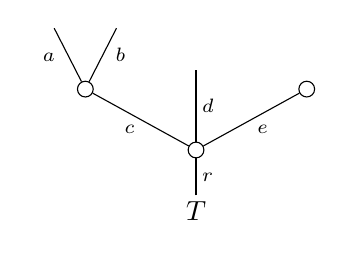
\begin{tikzpicture}[auto,grow=up, level distance = 2.2em,
	every node/.style={font=\scriptsize,inner sep = 2pt}]%
	\tikzstyle{level 2}=[sibling distance=4em]%
	\tikzstyle{level 3}=[sibling distance=2.25em]%
            \node [font=\normalsize] {$T$}
            child{node [dummy] {}
              child{node [dummy] {}
                edge from parent node [swap] {$e$}
              }
              child[level distance = 2.9
              em]{edge from parent node [swap] {$d$}}
              child{node [dummy] {}
                child{edge from parent node [near end, swap] {$b$}}
                child{edge from parent node [near end] {$\phantom{b}a$}}
                edge from parent node {$c$}
              }
              edge from parent node [swap] {$r$}
            };        
      \end{tikzpicture}
\end{equation}
Edges with no vertices $\circ$ above them are called \textit{leaves}, the unique bottom edge is called the \textit{root},
and edges that are neither are called \textit{inner edges}.
In the example above, $a$, $b$ and $d$ are leaves, $r$ is the root, and $c$ and $e$ are inner edges.
The sets of edges, inner edges, and vertices of a tree $T$ are denoted 
$\boldsymbol{E}(T)$, 
$\boldsymbol{E}^{\mathsf{i}}(T)$, 
and $\boldsymbol{V}(T)$, respectively.


Describing the maps in $\Omega$ requires some care.
To do so, we recall the algebraic notion of
a \emph{broad poset},
originally due to Weiss \cite{Wei12}
and further developed in \cite{Per18}.
%
For each edge $t$ in a tree topped by a vertex $\circ$, we write
$t^{\uparrow}$
for the tuple of edges immediately above $t$.
In \eqref{eq:TREE} one has  
$r^{\uparrow} = cde$, 
$c^\uparrow = ab$, 
and $e^\uparrow = \epsilon$,
where $\epsilon$ denotes the empty tuple.
We then encode each vertex symbolically as
$t^{\uparrow} \leq t$,
which we call a 
\emph{generating broad relation}.
This notation is motivated by a form of transitivity.
For example,
in \eqref{eq:TREE}
the relations
$cde \leq r$ and $ab \leq c$
generate, under \emph{broad transitivity},
the relation $abde \leq r$,
and one may similarly obtain relations
$cd \leq r$ and $abd \leq r$.
These relations, together with identity relations $t \leq t$,
then form the \emph{broad poset associated with $T$}
(alternatively, this broad poset data
is essentially equivalent to the data of
the colored operad $\Omega(T)$ associated to $T$, 
cf. \cite[\S 3]{MW07},
\cite[Rem. 4.4]{Per18}
or \eqref{TAUNER EQ}).


A map of trees $\varphi \colon S \to T$
in $\Omega$ is then an underlying map
of edge sets 
$\varphi \colon \boldsymbol{E}(S) \to \boldsymbol{E}(T)$
which preserves broad relations.



If an edge $t$ is pictorially above (or equal to) an edge $s$, we write $t \leq_d s$.
Equivalently, $t \leq_d s$ if there exists a broad relation $s_1\dots s_n \leq s$ such that $t = s_i$ for some $i$.
\\

Moreover,
our discussion will be simplified by assuming 
that $\Omega$ has exactly one representative of 
each \emph{planarized tree},
by which we mean a tree together with a planar representation as in \eqref{eq:TREE}
(alternatively, 
planarizations can be formalized as
suitable extensions of $\leq_d$ to a total order
\cite[\S 3.1]{BP_geo}).
Importantly, this implies that each map  
$\varphi \colon S \to T$ in $\Omega$
has a (strictly) unique factorization
$S \xrightarrow{\simeq} S' \to T$
as an isomorphism followed by a \emph{planar map}
\cite[Prop. 3.24]{BP_geo}.
Informally, $S'$ is obtained by giving $S$ the planarization ``pulled back'' from $T$.
Note that, 
in particular, the subcategory of planar maps is skeletal,
i.e. the only planar isomorphisms are the identities.




\begin{notation}
	We write $\eta$ for the \textit{stick} tree, the unique tree with a single edge and no vertices.
\end{notation}




\begin{example}\label{TREEMAP_EX}
	The edge labels in each tree $S_i$ below determine maps
	$\boldsymbol{E}(S_i) \to \boldsymbol{E}(T)$,
	where $T$ is as in \eqref{eq:TREE}.
	For $i \leq 4$ this encodes maps
	$S_i \to T$ in $\Omega$,
	but not for $i=5$.
\begin{equation}
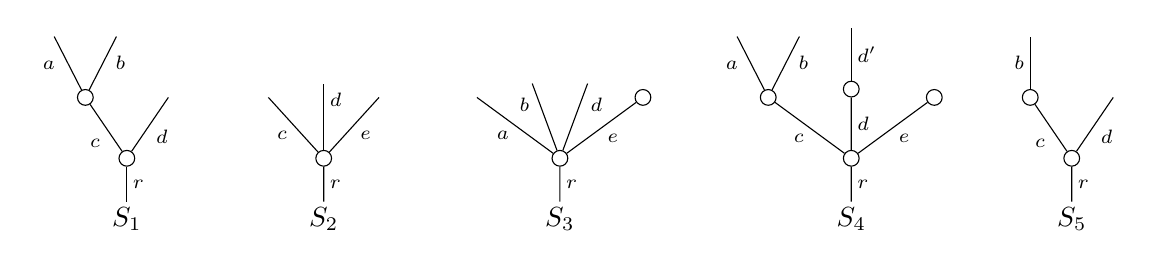
\begin{tikzpicture}[auto, grow=up, level distance = 2.2em,
	every node/.style={font=\scriptsize,inner sep = 2pt}]
\tikzstyle{level 2}=[sibling distance=3em]%
\tikzstyle{level 3}=[sibling distance=2.25em]%
	\node at (0,0) [font=\normalsize] {$S_1$} % 
                  child{node [dummy] {}
                    child{edge from parent node [swap] {$d\phantom{c}$}}
                    child{node [dummy] {}
                      child{edge from parent node [near end, swap] {$b$}}
                      child{edge from parent node [near end] {$\phantom{b}a$}}
                      edge from parent node {$\phantom{d}c$}
                    }
                    edge from parent node [swap] {$r$}
                  };
\tikzstyle{level 2}=[sibling distance=2em]%
	\node at (2.5,0) [font=\normalsize] {$S_2$} %
                  child{node [dummy] {}
                    child{edge from parent node [swap] {$e$}}
                    child [level distance = 2.7em] {edge from parent node [swap,near end] {$d$}}
                    child{edge from parent node {$c$}}
                    edge from parent node [swap] {$r$}
                  };
	\node at (5.5,0) [font=\normalsize] {$S_3$} 
                  child{node [dummy] {}
                    child{node [dummy] {}
                      edge from parent node [swap] {$e\phantom{a}$}
                    }
                    child [level distance = 2.7em]{edge from parent node [swap, very near end] {$d$}}
                    child [level distance = 2.7em]{edge from parent node [very near end] {$b$}}
                    child{edge from parent node {$\phantom{e}a$}}
                    edge from parent node [swap] {$r$}
                  };
\tikzstyle{level 2}=[sibling distance=3em]%
	\node at (9.2,0) [font=\normalsize] {$S_4$} 
                  child{node [dummy] {}
                    child{node [dummy] {}
                      edge from parent node [swap] {$e$}
                    }
                    child[level distance = 2.5em]{node [dummy] {}
                      child[level distance = 2.2em]{edge from parent node [swap] {$d'$}}
                      edge from parent node [swap] {$d$}
                    }
                    child{node [dummy] {}
                      child{edge from parent node [swap,near end] {$b$}}
                      child{edge from parent node [near end] {$\phantom{b}a$}}
                      edge from parent node {$c$}
                    }
                    edge from parent node [swap] {$r$}
                  };                    
	\node at (12,0) [font=\normalsize] {$S_5$}
                  child{node [dummy] {}
                    child{edge from parent node [swap] {$d\phantom{c}$}}
                    child{node [dummy] {}
                      child{edge from parent node {$b$}}
                      edge from parent node {$\phantom{d}c$}
                    }
                    edge from parent node [swap] {$r$}
                  };
\end{tikzpicture}
\end{equation}
\end{example}


A map of trees $\varphi \colon S \to T$ is called:
\begin{itemize}
\item a \textit{tall map} if
      $\varphi(\underline{l}_S) = \underline{l}_T$ and $\varphi(r_S) = r_T$,
      with $\underline{l}_{(-)}$ and $r_{(-)}$ denoting the tuple of leaf edges and the root edge;
\item a \textit{face map} if it is injective on edges;
      an \textit{inner face} if it is also tall; and
      an \textit{outer face} if, for any factorization
      $\varphi \simeq \varphi_1\varphi_2$
      with $\varphi_1,\varphi_2$ face maps
      and $\varphi_2$ inner, 
      $\varphi_2$ is an isomorphism;
%       it does not
%      admit a factorization as a non-isomorphism inner face followed by a face map;
\item a \textit{degeneracy} if it is surjective on edges and preserves leaves
      (and is thus tall).
\end{itemize}

Pictorially, inner face maps 
$S \to T$ remove some edges in $T$
(and merge the vertices adjacent to those edges),
outer face maps remove some vertices of $T$,
and degeneracies collapse some of the unary vertices of $S$.


\begin{example}
	In Example \ref{TREEMAP_EX},
	$S_1 \to T$ is an inner face, 
	$S_2 \to T$ is an outer face,
	$S_3 \to T$ is a face that is neither inner nor outer,
	and $S_4 \to T$ is a degeneracy.
\end{example}


\begin{notation}\label{MAPLABELS_NOT}
	In the remainder of \S \ref{EQTRDS SEC}
      we will label a 
      map in $\Omega$
      by the letters d/i/o/t/f/p
      to indicate that the map is
      a degeneracy/inner face/outer face/tall/face/planar.
\end{notation}


\begin{proposition}[{\cite[Prop. 2.2]{BP_edss}}]
      \label{NP_TREEFACT_PROP}
	A map of trees $\varphi \colon U \to V$ has a factorization, unique up to unique isomorphisms,
        \begin{equation}\label{NP_TREEFACT_EQ}
              S \xrightarrow{d} 
              S' \xrightarrow{i} 
              S'' \xrightarrow{o}
              T
        \end{equation}
        as a degeneracy followed by an inner face followed by an outer face.
\end{proposition}

\begin{remark}\label{TODF REM}
	A map $\varphi \colon S \to T$
	is tall (resp. a face)
	iff in the decomposition \eqref{NP_TREEFACT_EQ}
	the component labeled $o$ (resp. $d$)
	is an isomorphism.
	As such, by combining the 
	first two (resp. last two)
	maps in \eqref{NP_TREEFACT_EQ}
	one recovers the 
	``tall-outer face'' 
	(resp. ``degeneracy-face'')
	factorization of the map $\varphi$
	\cite[Prop. 3.36]{BP_geo}, \cite[Prop. 5.37]{Per18}.
\end{remark}



\begin{remark}\label{CNVXM REM}
	Following the previous remark, 
	it is natural to consider the class of maps
	$\varphi \colon S \to T$
	such that the inner face factor
	in \eqref{NP_TREEFACT_EQ} is an isomorphism.
	We call these maps \textit{convex},
	since they are readily seen to be 
	characterized by the following property:
	if $e <_d e' <_d e''$ in $T$ 
	and $e,e''$ are in the image of $\varphi$
	then so is $e'$.
	Notably, it follows from this characterization that convex maps are also closed under composition.
	
	Equivalently, $\varphi$ is convex precisely if
	the ``tall-outer face'' and ``degeneracy-face''
	factorizations coincide.
	In particular, outer faces are characterized
	as the convex faces.
\end{remark}


When accounting for planar structures,
one has the following refinement of 
Proposition \ref{NP_TREEFACT_PROP}.

\begin{proposition}[{cf. \cite[Prop. 2.2]{BP_edss}}]
      \label{TREEFACT_PROP}
      A map of trees $\varphi \colon U \to V$ has a strictly unique factorization
\begin{equation}\label{TREEFACT_EQ}
	S \xrightarrow{\simeq} 
	S_p \xrightarrow{pd} 
	\varphi S \xrightarrow{pi} 
	\overline{\varphi S} \xrightarrow{po} T
\end{equation}
	as an isomorphism followed by a planar degeneracy, a planar inner face, and a planar outer face.
\end{proposition}


\begin{remark}\label{TREEFACT_REM}
      The notation $\varphi S$ is motivated by the fact that this tree has edge set
      $\boldsymbol{E}(\varphi S) = \varphi (\boldsymbol{E}(S))$,
      while the 
      notation $\overline{\varphi S}$ is an instance of the 
      \emph{outer closure of an inner face}
      notation in \cite[Not. 2.14]{BP_edss}.
\end{remark}



\begin{remark}
	Generalizing Remarks \ref{TODF REM} and \ref{CNVXM REM},
	one has that, for any subset 
	$\mathcal{S} \subseteq \{\simeq,pd,pi,po\}$
	of the arrow labels 
	in \eqref{TREEFACT_EQ},
	the type of maps whose
	factors labeled by $\mathcal{S}$ are identities 
	is closed under composition.

	For example, the maps such that 
	the factors labeled $\simeq$ and $pi$
	are identities are the planar convex maps,
	while those maps such that
	the factors labeled $pd$ and $po$ 
	are identities are the 
	(possibly not planar) inner face maps.
	Both of these kinds of maps are closed under composition.	
\end{remark}


A \textit{corolla} is a tree with a single vertex.
We note that the subcategory of $\Omega$ spanned by corollas and isomorphisms is naturally identified with to the category $\Sigma$ of standard finite ordered sets
$\{1,2,\cdots,n\}$ and (non-ordered) isomorphisms.


%\begin{notation}
%      \label{LR_NOT}
%      For each $T \in \Omega$, there exists a unique corolla $\mathsf{lr}(T) \in \Sigma$ equipped with a planar tall map $\mathsf{lr}(T) \to T$,
%      which we call the \textit{leaf-root} of $T$.
%\end{notation}


Next, we recall the categories of (colored) forests used in 
\cite[Def. \ref{OC-COLFOR DEF}]{BP_FCOP}.


\begin{definition}\label{FOR DEF}
      The category $\Phi$ of \textit{forests} is the coproduct completion of the category $\Omega$ of trees:
      objects are formal coproducts 
      $F = \amalg_{i \in I} F_i$ with $F_i \in \Omega$,
      and an arrow 
      $\varphi \colon \amalg_{i \in I} F_i \to
      \amalg_{j \in J} F'_j$ is given by
      a map of indexing sets $\varphi \colon I \to J$ and
      maps $\varphi_i \colon F_i \to F'_{\varphi(i)}$ in $\Omega$ for each $i \in I$.

The sets of \emph{edges}, \emph{inner edges}, \emph{vertices}
of a forest $F = \amalg_i F_i$
are defined in the natural way as
\[
	\boldsymbol{E}(F)
	\simeq
	\amalg_i \boldsymbol{E}(F_i),
\qquad
	\boldsymbol{E}^{\mathsf{i}}(F)
	\simeq
	\amalg_i \boldsymbol{E}^{\mathsf{i}}(F_i),
\qquad
	\boldsymbol{V}(F)
	\simeq
	\amalg_i \boldsymbol{V}(F_i).
\]
\end{definition}


As with trees $T \in \Omega$, 
we assume that each forest $F = \amalg_{i \in I} F_i \in \Phi$
is planarized \cite[Def. 3.2 and Rem. 3.15]{BP_geo}, 
which is equivalent to choosing a total order of the indexing set $I$ and a planarization of each $F_i$.
Moreover, we similarly assume that $\Phi$ contains exactly one representative of each planarization,
so that the only planar isomorphisms are again the identities.

However, we caution that, in order to pullback a planarization
along $\varphi \colon F \to \tilde{F}$,
one needs to assume  
$\varphi$ sends roots of $F$
to $\leq_d$-incomparable edges of $\tilde{F}$, 
i.e. that $\varphi$ is an \emph{independent map}
\cite[Def. 5.28]{Per18}.
As such, in the context of forests our definition of 
planar map requires that the map is independent
\cite[Prop. 3.19]{BP_geo}.
In particular, the factorization
$F \xrightarrow{\simeq} F' \to \tilde{F}$
of a map $\varphi$ as an isomorphism followed by a planar map
exists only if $\varphi$ is independent
\cite[Prop. 3.24]{BP_geo}.


\begin{definition}\label{CFOREST_DEF}
      Let $\mathfrak C$ be a set of colors.
      The category $\Phi_{\mathfrak C}$ of \textit{$\mathfrak C$-forests} has:
      \begin{itemize}
      \item objects pairs $\vect F = (F, \mathfrak c)$ with
            $F \in \Phi$ a forest and
            $\mathfrak c \colon \boldsymbol{E}(F) \to \mathfrak C$ a coloring of its edges;
      \item arrows $\vect F = (F, \mathfrak c) \to (F', \mathfrak c') = \vect{F'}$ maps
            $\varphi \colon F \to F'$ in $\Phi$ such that $\mathfrak c = \mathfrak c' \varphi$.
      \end{itemize}      
	Lastly, we write
	$\Omega_{\mathfrak{C}} \subset \Phi_{\mathfrak{C}}$,
	which we call the category of 
	\emph{$\mathfrak{C}$-trees},
	for the full subcategory spanned by the objects 
	whose underlying forest is a tree,
	and 
	$\Sigma_{\mathfrak{C}} \subset \Omega_{\mathfrak{C}}$,
	which we call the category of 
	\emph{$\mathfrak{C}$-corollas},
	for the further subcategory of objects whose underlying tree is a corolla
	and whose maps are isomorphisms.
\end{definition}







\section{The dendroidal $W_!$-construction}
\label{WCONS AP}



In this paper we discuss the 
$W_!$-construction in the operadic context by extending the  
work of Dugger and Spivak in \cite{DS11} 
(which deals with the categorical context).

Our discussion will make systematic
use of the factorizations in $\Omega$ given by 
Proposition \ref{TREEFACT_PROP}.
We follow Notation \ref{MAPLABELS_NOT},
and label 
a map in $\Omega$
by either of the letters d/i/o/t/f/p
to indicate that the map is
a degeneracy/inner face/outer face/tall/face/planar.
Moreover, given a map $\phi\colon S \to T$,
we write
\[
	S \xrightarrow{d}
	\phi S \xrightarrow{i,p}
	\overline{\phi S} \xrightarrow{o,p}
	T
\]
for the (strictly) unique 
factorization of $\phi$ with the indicated properties
(cf. Remark \ref{TREEFACT_REM}).
% We note that the notation 
% $\phi(S)$ is motivated by the fact that this tree has edge set
% $\boldsymbol{E}(\phi S) = \phi (\boldsymbol{E}(S))$
% while the 
% $\overline{\phi S}$ notation is an instance of the 
% \emph{outer closure of an inner face}
% notation in \cite[Not. 2.14]{BP_edss}.



We now define the notion of dendroidal necklace,
generalizing the key notion in \cite{DS11}.
 

\begin{definition}[{cf. \cite[\S 3]{DS11}}]
	A \emph{necklace} is 
	a planar inner face map
	$\mathfrak{n} \colon J \to T$
	in $\Omega$.
	Moreover:
	%
	\begin{enumerate}[label = (\roman*)]
		\item 
		$J$ is called the \emph{inner face of joints} of the necklace;
		\item for each vertex $v \in \boldsymbol{V}(J)$,
		the outer face
		$\overline{\mathfrak{n} J_v} = T_v \hookrightarrow T$
		is called a \emph{bead} of the necklace.
	\end{enumerate}
\end{definition}

\begin{example}
      \label{NECKLACE_EX}
      Consider the trees $J$ and $T$ below.
      The labeling of the edges indicates a map $\boldsymbol{E}(J) \to \boldsymbol{E}(U)$ which
      encodes an inner face map.
      \begin{equation}
            \begin{tikzpicture}[auto,grow=up, level distance = 2.2em,
                  every node/.style={font=\scriptsize,inner sep = 2pt}]%
                  \tikzstyle{level 2}=[sibling distance=4em]%
                  \tikzstyle{level 3}=[sibling distance=2.25em]%
                  \node at (-5,0) [font=\normalsize] {$J$}
                  child{node [dummy,label=-120:$v$] {}
                    child{edge from parent node [swap] {$e$}
                    }
                    child{edge from parent node [swap] {$d$}}
                    child{node [dummy,label=left:$u$] {}
                      child{edge from parent node [near end] {$a$}} %{$\phantom{b}a$}
                      edge from parent node {$c$}
                    }
                    edge from parent node [swap] {$r$}
                  };        
                  \node [font=\normalsize] {$T$}
                  child{node [dummy] {}
                    child{node [dummy] {}
                      child{edge from parent node [swap] {$e$}}
                      edge from parent node [swap] {$f$}
                    }
                    child{edge from parent node [swap] {$d$}}
                    child{node [dummy] {}
                      child{node [dummy] {}
                        edge from parent node [near end, swap] {$b$}}
                      child{edge from parent node [near end] {$\phantom{b}a$}}
                      edge from parent node {$c$}
                    }
                    edge from parent node [swap] {$r$}
                  };        
            \end{tikzpicture}
      \end{equation}
      Here, $J = T - \set{b,f}$, and the two beads are
           \begin{equation}
            \begin{tikzpicture}[auto,grow=up, level distance = 2.2em,
                  every node/.style={font=\scriptsize,inner sep = 2pt}]%
                  \tikzstyle{level 2}=[sibling distance=4em]%
                  \tikzstyle{level 3}=[sibling distance=2.25em]%
                  \node at (-5,0) [font=\normalsize] {$\overline{\mathfrak n J_u} = T_u$}
                  child{node [dummy] {}
                    child{node [dummy] {}
                      edge from parent node [near end, swap] {$b$}
                    }
                    child{edge from parent node [near end] {$\phantom{b}a$}}
                    edge from parent node [swap] {$c$}
                  };
                  \node [font=\normalsize] {$\overline{\mathfrak n J_v} = T_v$}
                  child{node [dummy] {}
                    child{node [dummy] {}
                      child{edge from parent node [swap] {$e$}}
                      edge from parent node [swap] {$f$}
                    }
                    child{edge from parent node [swap] {$d$}}
                    child{edge from parent node {$c$}}
                    edge from parent node [swap] {$r$}
                  };        
            \end{tikzpicture}
      \end{equation}
\end{example}

In the following, we write 
$\mathsf{Face}_{sc}(J)$ for the \emph{Segal core poset} of $J$,
consisting of those planar outer faces with no inner edges
(which consist of either a single edge or a single vertex of $J$).



\begin{definition}
	Given a necklace $\mathfrak{n} \colon J \to T$ 
	we define its representable presheaf
	$\Omega[\mathfrak{n}] \in \mathsf{dSet}$ by
	\begin{equation}
	\Omega[\mathfrak{n}] 
	= 
	\underset{U \in \mathsf{Face}_{sc}(J)}{\colim}
	\Omega[\overline{\mathfrak{n} U}]
	=
	\bigcup_{U \in \mathsf{Face}_{sc}(J)} 
	\Omega[\overline{\mathfrak{n} U}]
	\end{equation}
	where the union formula is taken inside $\Omega[T]$.
	
	The category $\mathsf{Nec}$ of necklaces is then the full subcategory of $\mathsf{dSet}$
	spanned by the $\Omega[\mathfrak{n}]$.
\end{definition}



\begin{remark}
	The $\Omega[\mathfrak{n}]$ presheaves
	interpolate between the usual 
	Segal core and representable presheaves.
	More explicitly,
	each tree $T \in \Omega$
	gives rise to necklaces
	$T \xrightarrow{=} T$ and
	$\mathsf{lr}(T) \to T$
	for which
      \[
            \Omega[T \xrightarrow{=} T] = Sc[T],
            \qquad
            \Omega[\mathsf{lr}(T)] = \Omega[T].
      \]
In particular,
one obtains a natural inclusion
$\Omega \subset \mathsf{Nec}$
given by $T \mapsto \left( \mathsf{lr}(T) \to T \right)$.
%
However, we caution that the assignment
$T \mapsto Sc[T]$ is not functorial on $T$
(more precisely, it is functorial only with respect to \emph{convex} maps of trees,
in the sense of Remark \ref{CNVXM REM}).
\end{remark}



\begin{remark}
	In the context of linear trees,
	a necklace is an injective map
	$\mathfrak{n} \colon [n] \to [m]$,
	with beads $[m_i], 1 \leq n$
	such that $m_1 + \dots + m_k = m$.
	One then has an identification
	$\Omega[\mathfrak n] =
	\iota_!(\Delta[m_1] \vee \dots \vee \Delta[m_k])$
	where each $\vee$ symbol
	indicates that the last edge of 
	$\Delta[m_i]$ is identified with the first edge of
	$\Delta[m_{i+1}]$,
	thus recovering the original definition of necklace 
	due to Dugger-Spivak \cite[\S 1]{DS11}.
\end{remark}



\begin{lemma}\label{FACEINNECK LEM}
	Let $\mathfrak{n} \colon J \to T$ be a necklace. Then
	\begin{enumerate}[label=(\roman*)]
		\item a face $U \hookrightarrow T$
		is in $\Omega[\mathfrak{n}]$
		iff its outer closure $\bar{U}$ is; 
		\item an outer face 
		$U = \bar{U} \hookrightarrow T$
		is in $\Omega[\mathfrak{n}]$ iff 
		$\boldsymbol{E}^{\mathsf{i}}(J) \cap 
		\boldsymbol{E}^{\mathsf{i}}(U) = \emptyset$;
		\item there is a decomposition
		$
		\boldsymbol{E}(T) = 
		\boldsymbol{E}(J) \amalg 
		\coprod_{v \in \boldsymbol{V}(J)}
		\boldsymbol{E}^{\mathsf{i}}(T_v)
		$.
	\end{enumerate}
\end{lemma}



\begin{proof}
	(i) follows since $\Omega[\mathfrak{n}]$ is an union of outer faces.
	
	The arguments for (ii),(iii) are by induction on the number of inner edges $\boldsymbol{E}^{\mathsf{i}}(J)$,
	with the base case of $\boldsymbol{E}^{\mathsf{i}}(J) = \emptyset$  being obvious.
%	
	Otherwise, letting $e \in \boldsymbol{E}^{\mathsf{i}}(J)$, since $e$ is an inner edge of
	both $J$ and $T$
	one has grafting decompositions
	$J = J' \amalg_e J''$,
	$T = T' \amalg_e R''$
	together with inner face maps
	$\mathfrak{n}' \colon J' \to T'$,
	$\mathfrak{n}'' \colon J'' \to T''$.
%
	One then has that 
	$U$ is in $\Omega[\mathfrak{n}]$
	iff it is in either
	$\Omega[\mathfrak{n}']$ or in $\Omega[\mathfrak{n}'']$,
	yielding the induction step for (ii).
	The induction step for (iii) likewise follows. 
\end{proof}



\begin{remark}
	If $S \xrightarrow{d} S'$
	is a degeneracy,
	the vertices of $S'$ are naturally identified with
	the vertices of $S$ that are not collapsed to edges.
	Thus, by factoring a tall map
	$\varphi \colon S \xrightarrow{t} T$ as
	$S \xrightarrow{d} \varphi S \xrightarrow{i} T$
	the decomposition (iii) in Lemma \ref{FACEINNECK LEM}
	generalizes to 
\begin{equation}\label{EDGEBREAK EQ}
	\boldsymbol{E}(T) = 
	\boldsymbol{E}(\varphi S) \amalg 
	\coprod_{v \in \boldsymbol{V}(S)}
	\boldsymbol{E}^{\mathsf{i}}(\overline{\varphi S_v}).
\end{equation}
\end{remark}



\begin{notation}
	Given a necklace
	$\mathfrak{n} \colon J \to T$
	and outer face $F \to T$
	we write 
	$\mathfrak{n}_F \colon J_F \to F$
	for the necklace characterized by
\[
	\boldsymbol{E}^{\mathsf{i}}(J_F)
	=
	\boldsymbol{E}^{\mathsf{i}}(J)
	\cap
	\boldsymbol{E}^{\mathsf{i}}(F).
\]
\end{notation}

\begin{example}
      Let $\mathfrak n \colon J \to U$ be the necklace in Example \ref{NECKLACE_EX},
      and consider the outer faces $F$ and $F'$ of $T$ depicted below.
      Then $J_F$ is as depicted and $J_{F'} = F'$.
\begin{equation}
\begin{tikzpicture}[auto,grow=up, level distance = 2.2em,
                  every node/.style={font=\scriptsize,inner sep = 2pt}]%
\tikzstyle{level 2}=[sibling distance=4em]%
\tikzstyle{level 3}=[sibling distance=2.25em]%
	\node at (-10,0) [font=\normalsize] {$F$}
                  child{node [dummy] {}
                    child{node [dummy] {}
                      child{edge from parent node [swap] {$e$}}
                        edge from parent node [swap] {$f$}
                    }
                    child{edge from parent node [swap] {$d$}}
                    child{edge from parent node {$c$}}
                    edge from parent node [swap] {$r$}
                  };
	\node at (-5,0) [font=\normalsize] {$J_F$}
                  child{node [dummy] {}
                    child{edge from parent node [swap] {$e$}}
                    child{edge from parent node [swap] {$d$}}
                    child{edge from parent node {$c$}}
                    edge from parent node [swap] {$r$}
                  };     
	\node [font=\normalsize] {$F' = J_{F'}$}
                  child{node [dummy] {}
                    child{edge from parent node [swap] {$f$}}
                    child{edge from parent node [swap] {$d$}}
                    child{node [dummy] {}
                      child{edge from parent node [swap, near end] {$b$}}
                      child{edge from parent node [near end] {$a$}} % {{$\phantom{b}a$}}
                      edge from parent node {$c$}
                    }
                    edge from parent node [swap] {$r$}
                  };
\end{tikzpicture}
\end{equation}
In particular, note that one need not have a map $J_F \to J$
since $\boldsymbol{E}(J)$
may not contain $\boldsymbol{E}(J_F)$.
\end{example}



\begin{corollary}\label{NECINT COR}
	Let $\mathfrak{n} \colon J \to T$ be a necklace and
	$F \to T$ be an outer face.
	Then
\[
	\Omega[\mathfrak{n}_F] = \Omega[\mathfrak{n}] \cap \Omega[F]
\]
	where the intersection is taken inside
	$\Omega[T]$.
\end{corollary}

\begin{proof}
	Combining (i),(ii) in 
	Lemma \ref{FACEINNECK LEM}
	we see that a face $U \hookrightarrow F$ is
	in $\Omega[\mathfrak{n}]$
	iff $\boldsymbol{E}(J) \cap 
	\boldsymbol{E}^{\mathsf{i}}(\bar{U}) = \emptyset$,
	where (since $F$ is outer) the outer closure $\bar{U}$
	can be taken in either $T$ or $F$.
	But this is equivalent to 
	$\boldsymbol{E}(J_F) \cap 
	\boldsymbol{E}^{\mathsf{i}}(\bar{U}) = \emptyset$,
	i.e. to $U$ being in $\Omega[\mathfrak{n}_F]$.
\end{proof}



Before proceeding, we will need to better understand the maps in 
$\mathsf{Nec}$.





\begin{proposition}\label{MAPNECK PROP}
	Let $\mathfrak{n}\colon J \to T$ and $\mathfrak{n}' \colon J' \to T'$ be necklaces. Then:
\begin{enumerate}
\item[(i)]
	A map $\mathfrak{n} \to \mathfrak{n}'$ in $\mathsf{Nec}$
	is uniquely determined by some map 
	$T \to T'$ in $\Omega$. 
	More precisely, there exists an unique dashed arrow
	making the following commute.
\begin{equation}\label{NECKMAP EQ}
\begin{tikzcd}
	\Omega[\mathfrak{n}] 
	\ar[hookrightarrow]{r} 
	\ar{d}
&
	\Omega[T] 
	\ar[dashed]{d}{\exists !}
\\
	\Omega[\mathfrak{n}']
	\ar[hookrightarrow]{r}
&
	\Omega[T']
	\end{tikzcd}
\end{equation}
\item[(ii)]
	A map of trees 
	$\varphi \colon T \to T'$ in $\Omega$
	induces a map 
	$\mathfrak{n} \to \mathfrak{n}'$ in $\mathsf{Nec}$
	iff
	$\varphi J \supseteq J'_{\overline{\varphi T}}$.
\end{enumerate}
\end{proposition}


\begin{proof}
	We first address (i).
	The composite
	$\Omega[\mathfrak{n}] \to 
	\Omega[\mathfrak{n}'] \to 
	\Omega[T']$
	in \eqref{NECKMAP EQ}
	induces compatible maps
	$\Omega[\overline{\mathfrak{n} U}] \to \Omega[T']$
	in $\mathsf{dSet}$,
	and hence 
	compatible maps
	$\overline{\mathfrak{n} U} \to T'$ 
	in $\Omega$.
	Hence, the result follows from the identification
	$T
	\simeq  
	\underset{U \in \mathsf{Face}_{sc}(J)}{\colim}
	\overline{\mathfrak{n} U}$, where the colimit is now in $\Omega$,
	cf. \cite[Cor. 3.70]{BP_geo}.
	
	We now turn to (ii).
	By (i),(ii) in Lemma \ref{FACEINNECK LEM}
	the map $\varphi$ defines a map of necklaces 
	precisely if, 
	for each $v \in \boldsymbol{V}(J)$, one has
	\begin{equation}\label{MAPDES EQ}
	\emptyset
	=
	\boldsymbol{E}^{\mathsf{i}}(J')
	\cap
	\boldsymbol{E}^{\mathsf{i}}(\overline{ \varphi T_v})
	=
	\boldsymbol{E}^{\mathsf{i}}(J')
	\cap
	\boldsymbol{E}^{\mathsf{i}}(\overline{ \varphi J_v}).
	\end{equation}
	
	Writing $\tilde{\varphi}$ for the composite
	$
	J \to T \xrightarrow{\varphi} \overline{\varphi T}
	$
	and noting that $\tilde{\varphi}$ is tall,
	\eqref{EDGEBREAK EQ} becomes 
	\begin{equation}\label{DECOMPPR EQ}
	\boldsymbol{E}(\overline{\varphi T})
	=
	\boldsymbol{E}(\varphi J)
	\amalg
	\coprod_{v \in \boldsymbol{V}(J)}
	\boldsymbol{E}^{\mathsf{i}}(\overline{\varphi J_v}).
	\end{equation}
	Thus \eqref{MAPDES EQ}
	amounts to
	$\boldsymbol{E}^{\mathsf{i}}(J') \cap 
	\boldsymbol{E}(\overline{\varphi T})
	\subseteq
	\boldsymbol{E}(\varphi J)$,
	which is equivalent to the desired
	$\varphi J \supseteq J'_{\overline{\varphi T}}$
	(as these trees have the same outer edges).
\end{proof}



\begin{remark}\label{NECKMAPCHAR REM}
	Let $\mathfrak{n},\mathfrak{n}',T,T'$ be as in
	Proposition \ref{MAPNECK PROP}
	and suppose 
	$\varphi \colon T \to T'$
	defines a map
	$\mathfrak{n} \to \mathfrak{n}'$.
	Then for every outer face $F \to T$
	it follows from 
	Corollary \ref{NECINT COR}
	that the restriction 
	$F \to \overline{\varphi F}$
	likewise induces a restriction
	$\mathfrak{n}_F \to \mathfrak{n}'_{\overline{\varphi F}}$,
	from which it follows that
	$\varphi J_F \supseteq 
	\left(J'_{\overline{\varphi T}}\right)_{\overline{\varphi F}}
	=
	J'_{\overline{\varphi F}}$.
\end{remark}





\begin{remark}\label{BEADMAP REM}
	Let $\mathfrak{n} = (J \to T)$,
	$\mathfrak{n}^{\**} = (J^{\**} \to T^{\**})$
	be necklaces,
	and $\varphi \colon T \to T^{\**}$
	be a face map which induces a map of necklaces
	$\mathfrak{n} \to \mathfrak{n}^{\**}$.

	Then for each bead $T_{v} \hookrightarrow T$
	of $\mathfrak{n}$
	there is a unique bead
	$T^{\**}_{\varphi_{\**} v} \hookrightarrow T^{\**}$
	of $\mathfrak{n}^{\**}$
	such that
	$T_v \hookrightarrow T \to T^{\**}$
	factors as
	$T_v \to T^{\**}_{\varphi_{\**}v} \hookrightarrow T^{\**}$.
%	
	In particular, 
	this defines a map of sets of beads
	$\varphi_{\**} \colon 
	B(\mathfrak{n}) \to B(\mathfrak{n}^{\**})$.
\end{remark}



\begin{definition}\label{NWTNS DEF}
	Let $T \in \Omega$ be a tree.
	We define 
	$W(T) \in \mathsf{sOp}$
	to be the operad whose nerve is the preoperad
	$NW(T)$ with $n$-simplices given by
\[
	\left(NW(T)_n\right)_{\mathfrak{s}}(S)
=
	\left\{
	\text{factorizations }
	S \xrightarrow{t} 
	J_0 \xrightarrow{i,p} 
	J_1 \xrightarrow{i,p} 
	\cdots \xrightarrow{i,p}
	J_n \xrightarrow{f,p}
	T
	\text{ in $\Omega$}
	\right\}
\]
	if $\mathfrak{s} \colon \boldsymbol{E}(S) \to \boldsymbol{E}(T)$
	defines a map $\phi \colon S \to T$ in $\Omega$
	and
	$\left(\left(NW(T)\right)_n\right)_{\mathfrak{s}}(S) = \emptyset$
	otherwise.
	
	Alternatively, it suffices to require that all maps
	$S \to F_i$ are tall
	and all maps $J_i \to T$ are planar face maps.

	
	The functoriality of 
	$NW(T)$
	with respect to a map $(S', \mathfrak s') \to ({S},\mathfrak{s})$
	is described by the diagram
\[
\begin{tikzcd}
	S' \ar{r}{t} \ar{d}
&
	J'_0 \ar{r}{i,p} \ar{d}{o}
&
	J'_1 \ar{r}{i,p} \ar{d}{o}
&
	\cdots \ar{r}{i,p}
&
	J'_n \ar{r}{f,p} \ar{d}{o}
&
	T \ar[equal]{d}
\\
	S \ar{r}{t} 
&
	J_0 \ar{r}{i,p}
&
	J_1 \ar{r}{i,p}
&
	\cdots \ar{r}{i,p}
&
	J_n \ar{r}{f,p}
&
	T	
\end{tikzcd}
\]
	where 
	$S' \to J'_0 \to J_0$
	(resp. $J'_k \to J'_{k+1} \to J_{k+1}$)
	is defined as the ``tall followed by outer face''
	factorization of composite
	$S' \to S \to J_0$
	(resp. $J'_k \to J_{k} \to J_{k+1}$).

	More generally, 
	given a necklace $\mathfrak{n}\colon J \to T$,
	we define
	$NW(\mathfrak{n}) \subseteq NW(T)$
	as the subpresheaf
	of those factorizations with the property that
	$J_0 \supseteq J_{\overline{\phi S}}$.

	Note that the fact that this is a presheaf follows 
	since
\[
	\boldsymbol{E}^{\mathsf{i}}(J'_0)
=
	\boldsymbol{E}^{\mathsf{i}}(J_0)
	\cap
	\boldsymbol{E}^{\mathsf{i}}(\overline{\phi' S'})
\supseteq
	\boldsymbol{E}^{\mathsf{i}}(J_{\overline{\phi S}})
	\cap
	\boldsymbol{E}^{\mathsf{i}}(\overline{\phi' S'})
=
	\boldsymbol{E}^{\mathsf{i}}(J_{\overline{\phi' S'}}).
\]
\end{definition}



\begin{remark}
	Note that all
	$NW(\mathfrak{n})$ defined above are indeed nerves of operads,
	i.e., 
	$NW(\mathfrak{n})(\eta)$ is discrete
	and
	$NW(\mathfrak{n})$ satisfies the strict Segal condition
	(cf. \cite[Cor 3.69]{BP_geo}).
\end{remark}



Next, we discuss the functoriality of
$NW(T)$ with respect to $T \in \Omega$.

For each map $T \to T^{\**}$ in $\Omega$
we define
$\left(NW(T)\right)_{n,\mathfrak{s}}(S)
	\to 
\left(NW(T^{\**})\right)_{n,\mathfrak{s}^{\**}}(S)$
via the diagram
\begin{equation}\label{NWTTSTAR EQ}
\begin{tikzcd}
	S \ar{r}{t} \ar[equal]{d}
&
	J_0 \ar{r}{i,p} \ar{d}{d}
&
	J_1 \ar{r}{i,p} \ar{d}{d}
&
	\cdots \ar{r}{i,p}
&
	J_n \ar{r}{f,p} \ar{d}{d}
&
	T \ar{d}
\\
	S \ar{r}{t} 
&
	J^{\**}_0 \ar{r}{i,p}
&
	J^{\**}_1 \ar{r}{i,p}
&
	\cdots \ar{r}{i,p}
&
	J^{\**}_n \ar{r}{f,p}
&
	T^{\**}
\end{tikzcd}
\end{equation}
where
$J_n \to J^{\**}_n \to T^{\**}$
(resp. 
$J_{k-1} \to J^{\**}_{k-1} \to J^{\**}_k$)
is the "degeneracy followed by face"
factorization of the composite
$J_n \to T \to T^{\**}$
(resp.
$J_{k-1} \to J_{k} \to J^{\**}_k$).




\begin{proposition}
	For any map $T \to T^{\**}$ in $\Omega$, the induced map
	$\left(NW(T)\right)_{\mathfrak{s}}(S)
	\to 
	\left(NW(T^{\**})\right)_{\mathfrak{s}}(S)$
	in 
	\eqref{NWTTSTAR EQ}
	is functorial on $(S,\mathfrak{s})$.
\end{proposition}



\begin{proof}
	First, note that the composite
	$\left(NW(T)\right)_{\mathfrak{s}}({S})
	\to 
	\left(NW(T)\right)_{\mathfrak{s}'}({S'})
	\to 
	\left(NW(T^{\**})\right)_{\mathfrak{s}'}({S'})$
	is computed by the left diagram below,
	where
	$S' \to J'_i \to J_i$
	and 
	$J'_i \to \left(J_i'\right)^{\**} \to T^{\**}$
	are the unique factorizations with the indicated properties.
	On the other hand, the composite
	$\left(NW(T)\right)_{\mathfrak{s}}(S)
	\to 
	\left(NW(T^{\**})\right)_{\mathfrak{s}}(S)
	\to 
	\left(NW(T^{\**})\right)_{\mathfrak{s}'}(S')$
	is computed as on the right
	with 
	$J_i \to J^{\**}_i \to T'$ and
	$S' \to \left(J_i^{\**}\right)' \to J^{\**}_i$
	the unique indicated factorizations.
\begin{equation}
\begin{tikzcd}
	S \ar{r}{t} 
&
	J_i \ar{r}{f,p} 
&
	T \ar[equal]{d}
&&%%%
	S \ar{r}{t} \ar[equal]{d}
&
	J_i \ar{r}{f,p} \ar{d}{d}
&
	T \ar{d}
\\
	S' \ar{u} \ar{r}{t} \ar[equal]{d}
&
	J'_i \ar{r} \arrow{u}[swap]{o,p} \arrow{d}{d}
&
	T \ar{d}
&&%%%
	S \ar{r}
&
	J^{\**}_i \arrow{r}{f,p}
&
	T^{\**} \ar[equal]{d}
\\
	S' \ar{r}
&
	\left(J_i'\right)^{\**} \arrow{r}{f,p}
&
	T^{\**}
&&%%%
	S' \arrow{r}{t} \ar{u}
&
	\left(J_i^{\**}\right)' \ar{r} \arrow{u}[swap]{o,p}
&
	T^{\**}
\end{tikzcd}
\end{equation}
	The key to the proof is to show
	that the planar faces 
	$\left(J_i'\right)^{\**}$ and
	$\left(J_i^{\**}\right)'$
	of $T^{\**}$
	coincide, since it will then be automatic that all maps connecting the
	$\left(J_i'\right)^{\**}$ and
	$\left(J_i^{\**}\right)'$
	and $S'$, $T^{\**}$
	likewise match.

	To see this, we consider the following diagram.
\begin{equation}
\begin{tikzcd}
	S' \ar{r}{t} \ar{d}
&
	J'_i \ar{r} \ar{d}{o,p}
&
	T \ar[equal]{d}
\\
	S  \ar{r}{t} \ar[equal]{d}
&
	J_i \ar{r}{f,p}  \ar{d}{d}
&
	T \ar{d}
\\
	S \ar{r}
&
	J_i^{\**} \ar{r}{f,p}
&
	T^{\**}
\end{tikzcd}
\end{equation}
	Both faces  
	$\left(J'_i\right)^{\**}$ and 
	$\left(J^{\**}_i\right)'
	$
	can alternatively be built by factoring
	the composite 
	$J'_i \to J_i \to J_i^{\**}$,
	with 
	$\left(J'_i\right)^{\**}$ 
	coming from the 
	degeneracy-face factorization
	and 
	$\left(J^{\**}_i\right)'$
	coming from the 
	tall-outer factorization.
	But since 
	$J'_i \to J_i \to J_i^{\**}$
	is a composite of convex maps 
	(see Remark \ref{CNVXM REM})
	it is again convex, 
	so the two factorizations coincide, 
	finishing the proof.
\end{proof}



\begin{corollary}
	Let $\mathfrak{n} \colon J \to T$ and
	$\mathfrak{n}^{\**} \colon J^{\**} \to T^{\**}$
	be necklaces and suppose 
	$\psi \colon T\to T^{\**}$
	induces a map $\mathfrak{n} \to \mathfrak{n}^{\**}$.
%	
	Then the induced map
	$NW(T) \to NW(T^{\**})$
	restricts to a map
	$NW(\mathfrak{n}) \to NW(\mathfrak{n}^{\**})$.
\end{corollary}



\begin{proof}
	We need to show that the 
	map
	$NW(T) \to NW(T^{\**})$
	sends simplices such that
	$J_0 \supseteq 
	J_{\overline{\varphi S}}$
	to simplices such that
	$J^{\**}_0 \supseteq 
	J^{\**}_{\overline{\varphi^{\**} S}}$.
	This follows since
\[
	J^{\**}_0 = 
	\psi (J_0) \supseteq
	\psi (J_{\overline{\varphi S}})
	\supseteq
	J^{\**}_{\overline{\psi (\overline{\varphi S})}}
	=
	J^{\**}_{\overline{\varphi^{\**} S}}
\]	
where the third step is
Remark \ref{NECKMAPCHAR REM}.
\end{proof}



We now introduce a notation that plays an important role 
in two key technical results,
Propositions \ref{NECKCOL PROP} and 
\ref{NWKANEX_PROP}.
Recall that, for any tree 
$U \in \Omega$, 
the poset $\mathsf{Face}_{inn}(U)$
of planar inner faces is in fact a lattice,
with the join $F \vee F'$
the characterized by
$\boldsymbol{E}^{\mathsf{i}}(F \vee F') 
=
\boldsymbol{E}^{\mathsf{i}}(F)
\cup
\boldsymbol{E}^{\mathsf{i}}(F')$.

\begin{notation}\label{STAU NOT}
	Let $\mathfrak{n} \colon J \to T$
	be a necklace and $\phi\colon S \to T$ a map in $\Omega$.
	
	We write
	$S^{\mathfrak{n}} = \phi S \vee J_{\overline{\phi S}}$,
	where the join is 
	taken in $\mathsf{Face}_{inn}(\overline{\phi S})$.
\end{notation}

\begin{remark}\label{STAU REM}
	In the context of Notation \ref{STAU NOT}
	one has natural identifications
\begin{equation}
\begin{tikzcd}[column sep = 12pt]
	NW(\mathfrak{n})_{\phi}(S^{\mathfrak{n}}) 
	\ar{r}{\simeq}
&
	NW(\mathfrak{n})_{\phi}(S)
&
	NW(S^{\mathfrak{n}} \to \overline{\phi T})_{\phi}(S)
	\ar{l}[swap]{\simeq}
\end{tikzcd}
\end{equation}
induced by the natural maps
$S \to S^{\mathfrak{n}}$ between trees and 
$(S^{\mathfrak{n}} \to \overline{\phi T}) \to \mathfrak{n}$
between necklaces.
\end{remark}




\begin{proposition}\label{NECKCOL PROP}
	Let $\mathfrak{n} \colon J \to T$ be a necklace.
	Then one has an identification
\begin{equation}\label{NECKCOL EQ}
	W(\mathfrak{n})
	\simeq 
	\underset{U \in \mathsf{Face}_{sc}(J)}{\colim}
	W(T_U)
\end{equation}
	where the colimit takes place 
	in $\mathsf{sOp}$.
\end{proposition}



\begin{proof}
	We will verify \eqref{NECKCOL EQ}
	by working with nerves throughout.
	More explicitly, 
	we will show, that for any $X\in \mathsf{PreOp}$
	satisfying the strict Segal condition,
	giving a map
	$NW(\mathfrak{n}) \to X$
	is the same as giving compatible maps
	$NW(T_U) \to X$.

	Moreover, clearly both sides of 
	\eqref{NECKCOL EQ} yield $\boldsymbol{E}(T)$
	when evaluated on $\eta$.
	As such, we are free to fix throughout
	a map of colors $\boldsymbol{E}(T) \to X(\eta)$
	and verify the universal property 
	for maps respecting this color assignment.
	In particular, we are free to 
	evaluate $W(\mathfrak{n}),X$ on suitable 
	$\boldsymbol{E}(T)$-colored trees, 
	rather than on uncolored trees.

	Given maps $NW(T_U) \to X$
	we now define the map $NW(\mathfrak{n}) \to X$ via 
	(where $S^{\mathfrak{n}}$ is as in Notation \ref{STAU NOT})
\begin{equation}\label{LONGMAP EQ}
\begin{tikzcd}[column sep = 20pt, row sep=0]
	NW(\mathfrak{n})_{\mathfrak{s}}(S)
&
	NW(\mathfrak{n})_{\mathfrak{s}}(S^{\mathfrak{n}})
	\ar{l}[swap]{\simeq}{(I)}
	\ar{r}{\simeq}[swap]{(II)}
&
	\underset{b \in B( \mathfrak{n}_{\overline{\phi S}})}{\prod}
	NW(\mathfrak{n})_{\mathfrak{s}}(S^{\mathfrak{n}}_b)
\\
&&&
	\underset{b \in B( \mathfrak{n}_{\overline{\phi S}})}{\prod}
	NW(T_{\phi_{\**}b})_{\mathfrak{s}}(S^{\mathfrak{n}}_b)
	\ar{lu}[swap]{\simeq}{(III)}
	\ar{ld}{(IV)}
\\
	X_{\mathfrak{s}}(S)
&
	X_{\mathfrak{s}}(S^{\mathfrak{n}})
	\ar{r}{\simeq}[swap]{(V)}
	\ar{l}{(VI)}
&
	\underset{b \in B(\mathfrak{n}_{\overline{\phi S}})}{\prod}
	X_{\mathfrak{s}}(S^{\mathfrak{n}}_b)
\end{tikzcd}
\end{equation}
	where the arrows (II) and (V) are isomorphisms by the Segal condition
	while (III) is an isomorphism since 
	$S_b^{\mathfrak{n}} \to T$ factors through 
	$T_{\phi_{\**}b}$.
	
	Moreover, the arrow (IV) in \eqref{LONGMAP EQ}
	is induced by the chosen maps
	$NW(T_U) \to X$,
	so clearly 
	\eqref{LONGMAP EQ}
	denotes the only possible compatible map
	$NW(T) \to X$.

	It only remains to check that
	\eqref{LONGMAP EQ}
	is indeed a map in 
	$\mathsf{PreOp}$, i.e. that it is natural on 
	$\vect{S}=(S,\mathfrak{s})$.
	To see this, one first readily checks that a map
	$\psi \colon \vect{S} \to \vect{R}$
	induces a compatible inclusion
	$\psi \colon S^{\mathfrak{n}} \hookrightarrow R^{\mathfrak{n}}$
	showing the naturality of arrows (I),(VI) 
	in the zigzag.

	Next, by Remark \ref{BEADMAP REM}
	one has a map of bead sets
	$\psi_{\**} \colon 
	B(\mathfrak{n}_{\overline{\phi S}})
	\to
	B(\mathfrak{n}_{\overline{\phi' R}})$
	for which one has further compatible maps
	$S^{\mathfrak{n}}_b
	\to 
	R^{\mathfrak{n}}_{\psi_{\**}b}$,
	showing the naturality of the arrows (II),(V).
	Lastly, for any bead 
	$b \in B(\mathfrak{n}_{\overline{\phi S}})$
	one has
	$T_{\phi_{\**}b} = T_{\phi'_{\**} \psi_{\**}b}$
	showing naturality of the arrows (III),(IV).
\end{proof}





\begin{remark}\label{PREOPCOLEV REM}
	Let $I \xrightarrow{A_{\bullet}} \mathsf{PreOp}$
	be a diagram of preoperads and let
	$A = \colim_{i \in I} A_i$.
	
	For each $A(\eta)$-colored tree 
	$\vect{S} = (S,\mathfrak{s})$
	let us write
	$I_{\vect{S}/}$
	for the category whose objects are factorizations
	$\boldsymbol{E}(S) \to A_i(\eta) \to A(\eta)$ 
	for some $i \in I$,
	which we represent by 
	$\boldsymbol{E}(S) \to A_i(\eta)$,
	together with maps $i \to i'$ in $I$
	satisfying the obvious compatibility.
	
	Then
\begin{equation}\label{COLIMALT EQ}
	A_{\mathfrak{s}}(S) \simeq 
	\underset{(\boldsymbol{E}(S) \to A_i(\eta)) \in I_{\vect{S}/}}{\colim}
	A_{i,
	\mathfrak{s}_i}(S)
\end{equation}
	where in the expression 
	$A_{i,\mathfrak{s}_i}(S)$
	we write 
	$\mathfrak{s}_i$
	for the coloring given by
	$\boldsymbol{E}(S) \to A_i(\eta)$.
\end{remark}





\begin{proposition}
	\label{NWKANEX_PROP}
	Let $X \in \mathsf{dSet}$ and define
	$NW(X) \in \mathsf{PreOp}$ by
	\begin{equation}\label{NWKANEX EQ}
	NW(X) =
	\underset{(\mathfrak{n} \to X)
		\in \mathsf{Nec}_{/X}}{\colim}
	NW(\mathfrak{n}).
	\end{equation}
	where
	$\mathsf{Nec}_{/X} = \mathsf{Nec} \downarrow X$ is the over category of maps $\Omega[\mathfrak{n}] \to X$, and
	the colimit is taken in $\mathsf{PreOp}$.
	
	Then $NW(X)$ satisfies the strict Segal condition.
	%
	In particular, since $N$ is fully-faithful one has that
	$NW(X)$ is the nerve of the simplicial operad
\[
	W(X) =
	\underset{\Omega[\mathfrak{n}] \to X
	\in \mathsf{Nec}_{/X}}{\colim}
	W(\mathfrak{n}).
\]
	where the colimit is now taken in simplicial operads
	$\mathsf{sOp}$.
\end{proposition}



\begin{proof}
	We will evaluate 
	$NW(X)$ at each $X(\eta)$-colored tree
	$\vect{S}=(S,\mathfrak{s})$
	using Remark \ref{PREOPCOLEV REM}.
%	
	We write
	$\mathsf{Nec}_{\vect{S}//X}
	=
	\left(\mathsf{Nec}_{/X}\right)_{\vect{S}/}$
	for the category
	whose objects are pairs of arrows
	$\boldsymbol{E}(S) \to \Omega[\mathfrak{n}] \to X$
	whose composite is the coloring $\mathfrak{s}$.
	\eqref{COLIMALT EQ}
	then says that
\begin{equation}\label{NWKANEXEV EQ}
	NW(X)_{\mathfrak{s}}(S) 
	\simeq
	\underset{(\boldsymbol{E}(S) \to \Omega[\mathfrak{n}] \to X)
		\in \mathsf{Nec}_{\vect{S}//X}}{\colim}
	NW(\mathfrak{n})_{\mathfrak{s}_{\mathfrak{n}}}(S).
\end{equation}

	To show that $NW(X)$ satisfies the strict Segal condition, 
	we will rewrite \eqref{NWKANEXEV EQ} 
	by identifying appropriate subcategories of
	$\mathsf{Nec}_{\vect{S}//X}$.
	Firstly, write
	$\mathsf{Nec}_{\vect{S}//X}^{\Omega}
	\subset
	\mathsf{Nec}_{\vect{S}//X}$
	for the full subcategory of those objects for which the map
	$\boldsymbol{E}(S) \to \boldsymbol{E}(T)$
	defines a map $S \to T$ in $\Omega$.
		
	Additionally, we write 
	$
	\mathsf{Nec}_{\vect{S}//X}^{\Omega,nor}
	\subset
	\mathsf{Nec}_{\vect{S}//X}^{\Omega}
	$
	for the full subcategory of ``normalized factorizations'',
	which are defined by the property that
	$S \to T$ is a tall map and
	$J \supseteq \varphi(S)$.
	
	Moreover, there is a retraction
	$
	\mathsf{Nec}_{\vect{S}//X}^{\Omega}
	\xrightarrow{n}
	\mathsf{Nec}_{\vect{S}//X}^{\Omega,nor}
	$
	which sends
	$\boldsymbol{E}(S) \to \Omega[J \xrightarrow{\mathfrak{n}} T] \to X$
	to
	$n (\mathfrak{n}) = 
	(J_{\overline{\varphi S}} \vee \varphi S \to
	\overline{\varphi S})
	=
	(S^{\mathfrak{n}} \to \overline{\varphi S})
	$
	(cf. Notation \ref{STAU NOT}).
	Recall (cf. Remark \ref{STAU REM}) 
	that the natural map
	$n( \mathfrak{n}) \to \mathfrak{n}$ in $\mathsf{Nec}$
	induces isomorphisms
	$NW(n(\mathfrak{n}))_{\mathfrak{s}}(S) 
	\to
	NW(\mathfrak{n})_{\mathfrak{s}}(S)$.

	
	Since 
	$\mathsf{Nec}_{\vect{S}//X}^{\Omega}$
	is a cosieve of 
	$\mathsf{Nec}_{\vect{S}//X}$
	and 
	$NW(\mathfrak{n})_{\mathfrak{s}}(S) = \emptyset$
	whenever $\mathfrak{n}$ is not in 
	$\mathsf{Nec}_{\vect{S}//X}^{\Omega}$
	one can replace 
	$\mathsf{Nec}_{\vect{S}//X}$
	with 
	$\mathsf{Nec}_{\vect{S}//X}^{\Omega}$
	in
	\eqref{NWKANEXEV EQ}.
	Moreover, by the discussion in the previous paragraph one can
	likewise further replace it with
	$\mathsf{Nec}_{\vect{S}//X}^{\Omega,nor}$.
	
	Next, note that  the normalization conditions imply that
	$\mathsf{Nec}_{\vect{S}//X}^{\Omega,nor} 
	\simeq
	\prod_{v \in \boldsymbol{V}(S)}
	\mathsf{Nec}_{\vect{S_v}//X}^{\Omega,nor}$.
	Putting everything together we now obtain that
\begin{equation}
\begin{aligned}
	NW(X)_{\mathfrak{s}}(S) 
\simeq &
	\underset{(\boldsymbol{E}(S) \to \Omega[\mathfrak{n}] \to X)
		\in \mathsf{Nec}^{\Omega,nor}_{\vect{S}//X}}{\colim}
	NW(\mathfrak{n})_{\mathfrak{s}}(S)
\\
\simeq &
	\underset{(\boldsymbol{E}(S_v) \to \Omega[\mathfrak{n}_{T_v}] \to X)
		\in 
		\prod_{v \in \boldsymbol{V}(S)} \mathsf{Nec}^{\Omega,nor}_{\vect{S_v}//X}}{\colim}
	\left(\prod_{v \in \boldsymbol{V}(S)}
	NW(\mathfrak{n}_{T_v})_{\mathfrak{s}_v}(S_v)\right)
\\
\simeq &
	\prod_{v \in \boldsymbol{V}(S)}
	\left(
	\underset{(\boldsymbol{E}(S_v) \to \mathfrak{n}_{T_v} \to X)
		\in \mathsf{Nec}^{\Omega,nor}_{\vect{S_v}//X}}{\colim}
	NW(\mathfrak{n}_{T_v})_{\mathfrak{s}_v}(S_v)
	\right)
\\
\simeq &
	\prod_{v \in \boldsymbol{V}(S)} 
	NW(X)_{\mathfrak{s}_v}(S_v) 
\end{aligned}
\end{equation}
	where the second step is the identification above together with 
	the strict Segal condition on 
	$NW(\mathfrak{n})$,
	the third step is the fact that products commute with colimits in each variable, and the last step simply specifies
	the simplified version of \eqref{NWKANEXEV EQ}
	for $\vect{S_v} = (S_v,\mathfrak{s}_v)$.
	
	We have thus established the 
	strict Segal condition for $NW(X)$, 
	finishing the proof.
\end{proof}


\begin{remark}
	The normalization condition in the previous proof
	is equivalent to requiring that the tall map
	$\varphi \colon S \to T$
	induces a map
	$\mathsf{Sc}[S] \to \Omega[\mathfrak{n}]$.
\end{remark}



Propositions \ref{NECKCOL PROP} and 
\ref{NWKANEX_PROP}
now combine to give the following.


\begin{theorem}[{cf. \cite[Thm. 1.3]{DS11}}]
	\label{KANEXTCHAR THM}
	Consider the following diagram,
	were the functors labeled $W$ 
	are as defined by Definition \ref{NWTNS DEF}
	and Proposition \ref{NWKANEX_PROP}.
\begin{equation}
\begin{tikzcd}
	\Omega \ar[hookrightarrow]{r}
	\ar{rrd}[swap]{W} 
&
	\mathsf{Nec}
	\ar[hookrightarrow]{r}
	\ar{rd}{W}
&
	\mathsf{dSet}
	\ar{d}{W}
\\
&&
	\mathsf{sOp} 
\end{tikzcd}
\end{equation}
Then both triangles in this diagram are left Kan extensions.
%
In particular, the functor
$W \colon \mathsf{dSet} \to \mathsf{sOp}$
coincides with the functor
$W_! \colon \mathsf{dSet} \to \mathsf{sOp}$
as defined in \eqref{SOPDSET_EQ}.
\end{theorem}



\begin{remark}\label{TAUFUNEX REM}
	Recall that
	$\tau \colon \mathsf{dSet} \to \mathsf{Op}$
	is the left Kan extension along
	$\Omega \to \mathsf{dSet}$
	of the functor
	$\Omega \to \mathsf{Op}$
	given by $T \mapsto \Omega(T)$.
	
	It is then straightforward to check that
	that for any necklace
	$\mathfrak{n} = (J \to T)$
	one has 
	$\tau_! \Omega[\mathfrak{n}] \simeq \Omega(T)$.
	Adapting the proofs of 
	Proposition \ref{NWKANEX_PROP} and
	Theorem \ref{KANEXTCHAR THM} one then has
\begin{equation}
\begin{aligned}
	\left(N \tau_!X\right)_{\mathfrak{s}}(S) 
	\simeq &
\underset{(\boldsymbol{E}(S) \to 
	\Omega[J \to T] \to X)
	\in \mathsf{Nec}_{\vect{S}//X}}{\colim}
	\Omega[T]_{\mathfrak{s}}(S)
	\simeq &
\underset{(\boldsymbol{E}(S) \to 
	\Omega[J \to T] \to X)
	\in \mathsf{Nec}^{\Omega,nor}_{\vect{S}//X}}{\colim}
	\Omega[T]_{\mathfrak{s}}(S).
\end{aligned}
\end{equation}
Moreover, the normalization conditions guarantee
it is always 
$\Omega[T]_{\mathfrak{s}}(S) = \**$
in the rightmost formula.
Thus, specifying for the case of
$S=C$ a corolla one has that operations in
$\tau_!X(C)$
are represented by 
data of the form
$
	\Omega[C]
	\xrightarrow{t}
	\Omega[T]
	\leftarrow
	\Omega[J \to T]
	\to X
$
subject to the equivalence relation
generated by deeming two such data to be equivalent whenever there exists a map of necklaces
$(J \to T) \to (J^{\**} \to T^{\**})$
making the diagram below commute.
\[
\begin{tikzcd}
	\Omega[C] \ar{r}{t} \ar[equal]{d} &
	\Omega[T] \ar{d} &
	\Omega[J \to T] \ar{l} \ar{r} \ar{d} &
	X \ar[equal]{d}
\\
	\Omega[C] \ar{r}{t} &
	\Omega[T^{\**}] &
	\Omega[J^{\**} \to T^{\**}] \ar{l} \ar{r} &
	X
\end{tikzcd}
\]
\end{remark}




\begin{remark}\label{GTAUFUNEX REM}
	All the work in this appendix can be adapted to the categories
	$\mathsf{dSet}_G$ and $\mathsf{Op}_G$
	of genuine dendroidal sets and genuine operads
	discussed at the end of \S \ref{EDS_SEC}.
%	
	In particular, 
	the ``genuine operadification'' functor
	$\tau_G \colon \mathsf{dSet}_G \to \mathsf{Op}_G$
	first mentioned in
	\eqref{TAUFUNCTS EQ}
	can be described via an analogue of
	Remark \ref{TAUFUNEX REM}.
	
Briefly,
an \emph{equivariant necklace}
is a map $\mathfrak{n} \colon J \to T$ of $G$-trees
that is a planar orbital inner face.
Alternatively, this means that $\mathfrak{n}$
is an ordered isomorphism on roots/components which is a planar inner face on tree components. 
%
Then, just as in Remark \ref{TAUFUNEX REM}
one has that, for each $G$-corolla $C$,
the operations in 
$\tau_G X(C)$
can be represented by data
$\Omega[C] \xrightarrow{t,r}
\Omega[T] \leftarrow
\Omega[J \to T] \to 
X$
(where the map labeled $t,r$ induces an ordered isomorphism on roots which is tall in each component)
subject to the equivalence relation generated by diagrams
\[
\begin{tikzcd}
\Omega[C] \ar{r}{t,r} \ar[equal]{d} &
\Omega[T] \ar{d} &
\Omega[J \to T] \ar{l} \ar{r} \ar{d} &
X \ar[equal]{d}
\\
\Omega[C] \ar{r}{t,r} &
\Omega[T^{\**}] &
\Omega[J^{\**} \to T^{\**}] \ar{l} \ar{r} &
X.
\end{tikzcd}
\]

\end{remark}




The remainder of this appendix is dedicated to providing a more explicit description of $W(X)$ for $X \in \mathsf{dSet}$.
%
Combining the proof of Proposition \ref{NWKANEX_PROP}
with the description of the simplices 
in Definition \ref{NWTNS DEF} gives the following.

\begin{corollary}[{cf. \cite[Cor. 4.4]{DS11}}]
	\label{NWXREPS COR}
	Let $X\in \mathsf{dSet}$.
	Then the simplices in
	$NW(X)_{n,\mathfrak{s}}(S)$
	are equivalence classes of quadruples
	$(\mathfrak{n}, S \xrightarrow{\phi} T, \Omega[\mathfrak{n}] \xrightarrow{x} X, J_{\bullet})$ 
	where:
	\begin{enumerate}[label=(\roman*)]
		\item $(J \xrightarrow{\mathfrak{n}} T) \in \mathsf{Nec}$ is a necklace; 
		\item $S \xrightarrow{\phi} T$
		is a tall map in $\Omega$
		which induces a map
		$\mathsf{Sc}[S] \to \Omega[\mathfrak{n}]$,
		i.e.
		$J \supseteq \phi(S)$;		
		\item $\Omega[ \mathfrak{n}] \to X$ is a map in $\mathsf{dSet}$
		such that the induced composite
		$\boldsymbol{E}(S) \to 
		\boldsymbol{E}(T) \to X(\eta)$
		is the coloring $\mathfrak{s}$;
		\item $J_{\bullet}$ denotes a tall simplex in $NW(\mathfrak{n})_{n,\phi}$, i.e.
		a factorization of $\phi$	
	\begin{equation}\label{STRINCOR EQ}
	\begin{tikzcd}
		S \ar{r}{t}
	&
		J_0 \ar{r}{i,p}
	&
		J_1 \ar{r}{i,p}
	&
		\cdots
		\ar{r}{i,p}
	&
		J_n \ar{r}{i,p}
	&
		T
	\end{tikzcd}
	\end{equation}
		such that 
		$J_0 \supseteq J$.
	\end{enumerate}
The equivalence relation is generated by considering 
$(\mathfrak{n},\phi,x,J_{\bullet})$ and
$(\mathfrak{n}^{\**},\phi^{\**},x^{\**},J_{\bullet}^{\**})$
to be equivalent if there is
a map
$\varphi \colon \Omega[\mathfrak{n}] \to \Omega[\mathfrak{n}^{\**}]$
such that
$\phi^{\**} = \varphi \phi$,
$x = x^{\**} \varphi $
and
$J^{\**}_k = \varphi J_k$
(i.e $J^{\**}_{\bullet}$
is obtained by push forwarding 
$J_{\bullet}$ along $\varphi$
in the sense of \eqref{NWTTSTAR EQ}).
\end{corollary}


Our final goal in this appendix is to show that, 
among the representatives in 
Corollary \ref{NWXREPS COR}
one can always identify a nice representative that is 
suitably unique.

Firstly, we discuss uniqueness of 
the maps
$\Omega[\mathfrak{n}] \xrightarrow{x} X$ up to degeneracy.

\begin{definition}
	A map of necklaces 
	$(J\to T) \to (J^{\**} \to T^{\**})$
	is called a \emph{degeneracy}
	if the associated map
	$\varphi \colon T \to T^{\**}$
	is a degeneracy and
	$\varphi J = J^{\**}$.
\end{definition}


\begin{definition}[{cf. \cite[\S 4]{DS11}}]
	Let $J \xrightarrow{\mathfrak{n}} T$ be a necklace and 
	$X \in \mathsf{dSet}$.
	A map $\Omega[\mathfrak{n}] \to X$
	is called \emph{totally non-degenerate}
	if for all beads $T_v$ of $\mathfrak{n}$
	the induced dendrex
	$\Omega[T_v] \to X$
	is non-degenerate.
\end{definition}


\begin{lemma}[{cf. \cite[Prop. 4.7]{DS11}}]
	\label{DEGNECK LEM}
	Any map 
	$\Omega[\mathfrak{n}] \to X$
	has a factorization, unique up to unique isomorphism, as
\[
	\Omega[J \xrightarrow{\mathfrak{n}} T] \to 
	\Omega[J^{\**} \xrightarrow{\mathfrak{n}^{\**}} T^{\**}] \to X
\]
	where the first map is a degeneracy of necklaces
	and the second map is totally non-degenerate.
\end{lemma}



\begin{proof}
	The proof is by induction on the size of 
	$\boldsymbol{E}^{\mathsf{i}}(J)$.
	The base case is that of $\boldsymbol{E}^{\mathsf{i}}(J) = \emptyset$
	(note that then it must also be $\boldsymbol{E}^{\mathsf{i}}(J') = \emptyset$),
	in which case the result reduces to 
	\cite[Prop. 6.9]{CM11} or
	\cite[Prop. 5.62]{Per18}.

	Otherwise, let $e \in \boldsymbol{E}^{\mathsf{i}}(J)$
	and consider the grafting decomposition
	$T = R \amalg_e S$.
	By the induction hypothesis, 
	one has factorizations, unique up to unique isomorphism,
	$\Omega[\mathfrak{n}_{R}] \to \Omega[\mathfrak{n}_R'] \to X$,
	$\Omega[\mathfrak{n}_S] \to \Omega[\mathfrak{n}_{S}'] \to X$.
	Writing 
	$\mathfrak{n}_R' = (J'_R \to R')$
	and 
	$\mathfrak{n}_S' = (J'_S \to S')$,
	we then set
	$\mathfrak{n}'= \left(
	J'_R \amalg_e J'_S \to T'_R \amalg_e T'_S
	\right)$.
	The uniqueness up to unique isomorphism property of
	$tau'$ is easily seen to be inherited from 
	the analogue property for 
	$\mathfrak{n}'_R,\mathfrak{n}'_S$
	(note that the ``unique isomorphism'' clause
	implies that there is no ambiguity concerning the grafting edge $e$),
	finishing the proof.
\end{proof}


Next, we also need a preferred form for the tall simplex data in \eqref{STRINCOR EQ}.


\begin{definition}[{cf. \cite[\S 4]{DS11}}]
	A tall simplex as in 
	\eqref{STRINCOR EQ}
	is called \emph{flanked}
	if $J_0 = J$
	and $J_n = T$.
%	
	Further, a quadruple
	$(\mathfrak{n},\phi,x,J_{\bullet})$
	is called \emph{flanked} if $J_{\bullet}$ is.
\end{definition}


\begin{remark}
	Suppose $(\mathfrak{n},\phi,x,J_{\bullet})$
	is a flanked quadruple
	and set $\mathfrak{n}_k = (J_k \to T)$.
	Then the structure maps in \eqref{STRINCOR EQ}
	induce a diagram of necklace maps
\begin{equation}
\begin{tikzcd}[column sep=12pt]
	\mathsf{Sc}[T]
	\ar[equal]{r} 
&
	\Omega[\mathfrak{n}_n]
	\ar{r}
&
	\Omega[\mathfrak{n}_{n-1}]
	\ar{r}
&
	\cdots
	\ar{r}
&
	\Omega[\mathfrak{n}_0]
	\ar[equal]{r}
&
	\Omega[\mathfrak{n}]
&
	\mathsf{Sc}[S]
	\ar{l}
\end{tikzcd}
\end{equation} 
\end{remark}



\begin{remark}\label{FLNKNECDEG REM}
	If both simplices 
	$J_{\bullet},J^{\**}_{\bullet}$ in a pushforward diagram
	\eqref{NWTTSTAR EQ}
	are flanked,
	then the associated map of necklaces
	$\mathfrak{n} \to \mathfrak{n}^{\**}$
	is a degeneracy.
\end{remark}


In what follows we say a quadruple
$(\mathfrak{n},\phi,x,J_{\bullet})$
as in Corollary \ref{NWXREPS COR}
is \emph{flanked} if $J_{\bullet}$ is and
\emph{totally non-degenerate} if $x$ is.


\begin{lemma}[{cf. \cite[Lemma 4.5]{DS11}}]
	\label{FLANKING LEM}
	\begin{enumerate}[label=(\roman*)]
		\item Any quadruple $(\mathfrak{n},\phi,x,J_{\bullet})$
		as in Corollary \ref{NWXREPS COR} is equivalent a flanked one;
		\item if two flanked quadruples are equivalent, then the equivalence can be described via a zigzag involving only flanked quadruples.
	\end{enumerate}
\end{lemma}



\begin{proof}
	The key to the proof is the fact that 
	the map $J_n \to T$
	induces a map of necklaces
	$(J_0 \to J_n) \to (J \to T)$.
	This map of necklaces then induces a pushforward of simplices
\begin{equation}
\begin{tikzcd}
	S \ar{r}{t} \ar[equal]{d}
&
	J_0 \ar{r}{i,p} \ar[equal]{d}
&
	J_1 \ar{r}{i,p} \ar[equal]{d}
&
	\cdots
	\ar{r}{i,p}
&
	J_n \ar[equal]{r} \ar[equal]{d}
&
	J_n \ar{d}
\\
	S \ar{r}{t}
&
	J_0 \ar{r}{i,p}
&
	J_1 \ar{r}{i,p}
&
	\cdots
	\ar{r}{i,p}
&
	J_n \ar{r}{i,p}
&
	T
\end{tikzcd}
\end{equation}	
	where the top simplex (and thus the associated quadruple) is now flanked, so (i) follows.

	(ii) then follows by noting that the procedure above is natural.
	More precisely, 
	an arbitrary pushforward of tall simplices
	along the necklace map $(J,T) \to (J^{\**} \to T^{\**})$
	as in \eqref{NWTTSTAR EQ}
	induces a pushforward of flanked simplices
\begin{equation}
\begin{tikzcd}
	S \ar{r}{t} \ar[equal]{d}
&
	J_0 \ar{r}{i,p} \ar{d}{d}
&
	J_1 \ar{r}{i,p} \ar{d}{d}
&
	\cdots \ar{r}{i,p}
&
	J_n \ar[equal]{r} \ar{d}{d}
&
	J_n \ar{d}
\\
	S \ar{r}{t} 
&
	J^{\**}_0 \ar{r}{i,p}
&
	J^{\**}_1 \ar{r}{i,p}
&
	\cdots \ar{r}{i,p}
&
	J^{\**}_n \ar{r}{f,p}
&
	T^{\**}
\end{tikzcd}
\end{equation}
along the necklace map
$(J_0 \to J_n) \to (J^{\**}_0 \to J^{\**}_n)$.
\end{proof}



\begin{corollary}[{cf. \cite[Cor. 4.8]{DS11}}]
	Each quadruple $(\mathfrak{n},\phi,x,J_{\bullet})$ as in Corollary \ref{NWXREPS COR}
	has a representative, unique up to unique isomorphism,
	which is both flanked and totally non-degenerate.
\end{corollary}



\begin{proof}
	By Lemma \ref{FLANKING LEM}(i)
	any quadruple is equivalent to a flanked quadruple 
	and by Lemma \ref{DEGNECK LEM}
	any flanked quadruple is equivalent to a flanked quadruple that is also totally non-degenerate.
	
	As for the uniqueness condition, 
	by Lemma \ref{FLANKING LEM}(ii)
	we need only consider zigzags of 
	equivalences of flanked quadruples, 
	which are induced by necklace degeneracies, 
	cf. Remark \ref{FLNKNECDEG REM}.
	Thus, arguing by induction on the size of the zigzag,
	Lemma \ref{DEGNECK LEM} implies that 
	all flanked quadruples in the zigzag have the same
	totally non-degenerate quotient,
	so the desired uniqueness claim reduces to the uniqueness claim
	in Lemma \ref{DEGNECK LEM}.
\end{proof}



\begin{example}\label{WPARTIALT_EX}
	Let $U \in \Omega$ be a tree.
	We will apply Lemma \ref{FLANKING LEM} to describe
	$W_!(\partial \Omega[U])$.
	Firstly, 
	on any signature $\vect{C}$
	that is not isomorphic to the leaf-root signature
	one readily sees that
	$W_!(\partial \Omega[U])(\vect{C}) = W(U)(\vect{C})$.

	For the interesting case of 
	$W_!(\partial \Omega[U])(\underline{l};r)$,
	note that a map
	$\Omega[J \to V] \to \Omega [U]$
	is totally non-degenerate iff
	the inducing map $V \to U$
	is a face map. 
	Moreover, we are free to choose the unique planar representative.
	Next, note that 
	$\Omega[J \to V] \to \Omega [U]$
	factors through $\partial \Omega[U]$
	iff either $V \neq U$ or $J \neq \mathsf{lr}(U)$.
	In other words, the $n$-simplices of 
	$W_!(\partial \Omega[U])(\underline{l};r)$
	are uniquely represented by strings
\begin{equation}\label{WDELREP EQ}
	J_0 \xrightarrow{i,p} 
	J_1 \xrightarrow{i,p} 
	\cdots \xrightarrow{i,p}
	J_n = V \xrightarrow{i,p} U
\end{equation}
	such that either $J_n \neq U$ or $J_0 \neq \mathsf{lr}(U)$.
	
	Put another way, 
	$W_!(\partial \Omega[U])(\underline{l},r)$
	is the boundary of the nerve of the poset of inner faces
	$\mathsf{Face}_{inn}(U) \simeq 
	(0 \to 1)^{\times \boldsymbol{E}^{\mathsf{i}}(U)}$.
	In particular, 
	$W_!(\partial \Omega[U])(\underline{l},r)$ 
	is identified with the \emph{domain} of the iterated pushout product
	\[
	\left(
	\{0,1\} \to \Delta[1]
	\right)^{\square \boldsymbol{E}^{\mathsf{i}}(U)}.
	\]
\end{example}



\begin{example}\label{WPARTIALT2_EX}
	Let $U\in \Omega$ and 
	$\emptyset \neq E \subseteq \boldsymbol{E}^{\mathsf{i}}(U)$.
	Just as in Example \ref{WPARTIALT_EX}
	one has 
	$W_!(\Lambda^E[U])(\vect{C}) = W(U)(\vect{C})$
	whenever $\vect{C} \not \simeq (\underline{l};r)$
	(though we note that this fails for outer horns).

	Then, one has that 
	$\Omega[J \to V] \to \Omega[U]$
	factors through $\Lambda^E[U]$
	iff either $V \not \supseteq U-E$ or $J \neq \mathsf{lr}(U)$.
	I.e., the $n$-simplices of
	$W_!(\Lambda^E[U])(\underline{l};r)$ 
	are uniquely represented by strings 
	\eqref{WDELREP EQ}
	such that either 
	$J_n \not \supseteq U-E$ or
	$J_0 \neq \mathsf{lr}(U)$. 
	Put another way, 
	$W_!(\Lambda^E[U])(\underline{l},r)$ 
	is identified with the \emph{domain} of
	the iterated pushout product
\[
	\left(
	\{0,1\} \to \Delta[1]
	\right)^{\square \boldsymbol{E}^{\mathsf{i}}(U)-E}
	\square
	\left(
	\{1\} \to \Delta[1]
	\right)^{\square E}.
\]
\end{example}



\section{Conclusions}

In the categorical setting
the left adjoint $W_!$ admits 
an explicit description, due to Dugger and Spivak \cite{DS11},
in terms of so called \emph{necklaces},
which we extend to the operadic setting in 
Appendix \ref{WCONS AP}.
We now summarize the results in that appendix we will need.



For a tree $U \in \Omega$ there is 
a simplicial operad
$W(U) \in \mathsf{sOp}$
with set of colors $\boldsymbol{E}(U)$
and whose $n$-simplices evaluated at
a $\boldsymbol{E}(U)$-corolla
$\vect{C} = (C,\mathfrak{c})$


\begin{equation}\label{WU_EQ}
	W(U)_n(\vect C) =
	\begin{cases}
	\left\{\text{factorizations }
	C \xrightarrow{t} 
	F_0 \xrightarrow{i,p} 
	\cdots \xrightarrow{i,p}
	F_n \xrightarrow{f,p} U
	\right\}
&
	\mbox{if $\boldsymbol{E}(C) \xrightarrow{\mathfrak{c}} \boldsymbol{E}(U)$ defines a map in $\Omega$}
\\
	\varnothing
&
	\mbox{otherwise.}
\end{cases}
\end{equation}
where we label maps in $\Omega$ as
$t/i/f/p$
to indicate they are 
tall/inner faces/faces/planar
(cf. \S \ref{FORESTS_SEC}).


\begin{remark}
	The factorization description in \eqref{WU_EQ}
	reflects our approach in Appendix \ref{WCONS AP},
	which makes heavy use of the factorizations in 
	Proposition \ref{TREEFACT_PROP}.
	However, there is a simpler and more familiar description of $W(U)(\vect{C})$.
	If one lets
	$C \xrightarrow{t} U_C \xrightarrow{o,p} U$
	denote the unique ``tall followed by planar outer face'' factorization, 
	repeated use of Proposition \ref{TREEFACT_PROP}
	shows that the 
	$F_0 \to \cdots \to F_n$
	strings in \eqref{WU_EQ}
	are precisely the strings of planar inner faces of $U_C$.
	And since the latter are in bijection with strings of subsets of inner edges $\boldsymbol{E}^{\mathsf{i}}(U_C)$, 
	we have 
\begin{equation}\label{WU_EQ2}
	W(U)(\vect C) =
	\begin{cases}
	\Delta[1]^{\times \boldsymbol{E}^{\mathsf{i}}(U_{C})}
	\qquad
&
	\mbox{if $\boldsymbol{E}(C) \xrightarrow{\mathfrak{c}} \boldsymbol{E}(U)$ defines a map in $\Omega$}
\\
\varnothing
&
	\mbox{otherwise,}
	\end{cases}
\end{equation}
which recovers the description in \cite[\S 4]{CM13b}.
\end{remark}



\begin{remark}
	One neat feature of the description in 
	\eqref{WU_EQ}
	is that the nerve $N W(U)$
	can be defined identically 
	(cf. Definition \ref{NWTNS DEF}),
%	It is then straightforward to check that the nerve thus defined has the required functoriality and satisfies the strict Segal condition.
	allowing us to deduce many properties of $W_!$
	via systematic use of 
	Proposition \ref{TREEFACT_PROP}.
\end{remark}













\bibliography{biblio3}{}
\bibliographystyle{amsalpha2}



\end{document}


%%% Local Variables:
%%% mode: latex
%%% TeX-master: t
%%% End:
